\icode[purple]{E-EMM-SI-L4-260928-001}
如图所示，某同学为探究带电粒子“约束”问题，构想了垂直纸面向里的匀强磁场区域，磁感应强度为\(B\)，边界分别是半径为\(R\) 和\(2R\)的同心圆，\(O\)为圆心，\(A\)为磁场内在圆弧上的点且\(OP = PA\)。若有一粒子源垂直方向在纸面内的\,\qty{360}{\degree}发射出比荷为\(\frac{q}{m}\)的带负电粒子，速度连续分布且无相互作用，不计重力，\(\sin\) \,\qty{37}{\degree}=0.6。对粒子源的位置和被约束相关量的说法正确的是\paren[]

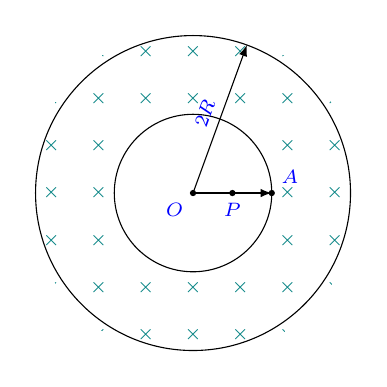
\begin{tikzpicture}[>=latex,font=\scriptsize]
    \clip (0,0) circle(2.1);
    \foreach \x in{-1.8,-1.2,...,2}
        \foreach \y in{-1.8,-1.2,...,2}
            \node at(\x,\y)[teal]{\( \times \)};
    \draw (0,0) circle(2);
    \filldraw[fill=white,draw=black] (0,0) circle(1);
    \fill (0,0) circle(.04) (.5,0)node[below,blue]{\(P\)} circle(.04) (1,0) circle(.04);
    \draw[->] (0,0)--node[above,rotate=70,blue]{\(2R\)}(70:2);
    \draw[->] (0,0)node[below left,blue]{\(O\)}--(1,0)node[above right,blue]{\(A\)};
\end{tikzpicture}
\begin{choices}
    \item 在\(A\)时，被磁场约束的粒子速度最大值\(v_{mA} = \frac{3qBR}{2m}\)
    \item 在\(O\)时，被磁场约束的粒子速度最大值\(v_{mO} = \frac{3qBR}{2m}\)
    \item 在\(O\)时，被磁场约束的粒子每次经过磁场时间最大值\(t_m = \frac{127\pi m}{90qB}\)
    \item 在\(P\)时，被磁场约束的粒子速度最大值\(v_{mP} = \frac{qBR}{m}\)
\end{choices}
\begin{answer}
    
    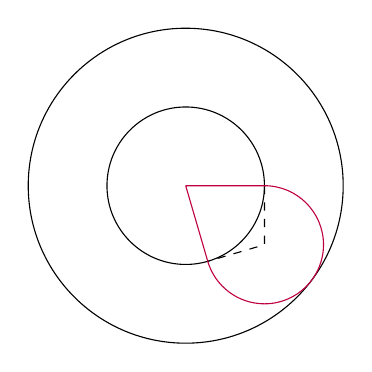
\begin{tikzpicture}
        \draw (0,0) circle(2) (0,0) circle(1);
        \draw[dashed] (1,0)--(1,-.75)--(-74:1);
        \draw[purple] (0,0)--(1,0) arc(90:-164:.75)--(0,0);
    \end{tikzpicture}
\end{answer}